\section{Integracja systemu}

Ostatecznym etapem projektu było połączenie stworzonych w~ten sposób modułów w~ramach pojedynczego bloku języka VHDL. Ze względu na regularne testowanie wdrażanych elementów oraz z~góry przemyślaną strukturę projektu proces ten przebiegł bezpoleśnie. Ostatecznie projekt udało się zsyntezować oraz przejść przez etap wirtualnej implementacji, czego efekt przedstawia Rys. \ref{synthesis}.

\vspace{1cm}
\begin{figure}[ht]
    \centering
    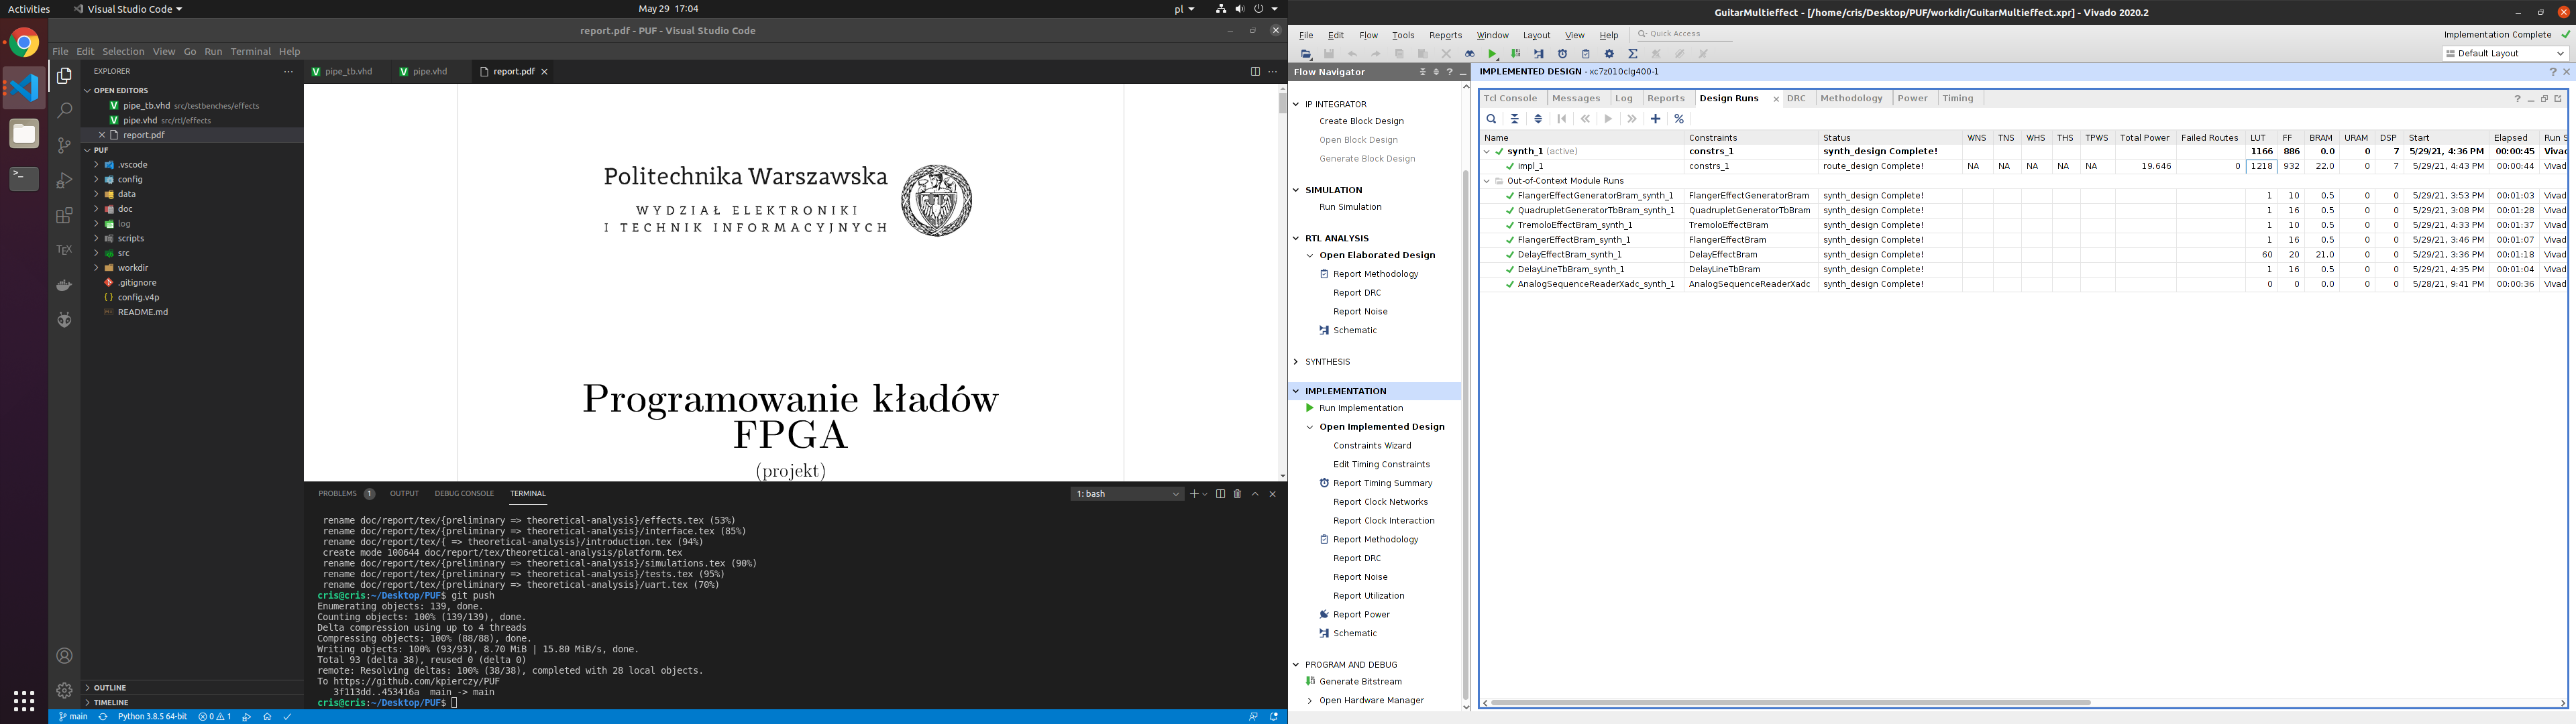
\includegraphics[width=\textwidth]{img/implementation.png}
    \captionsetup{format=plain,justification=centering}
    \caption{Efekt syntezy projektu}
    \label{synthesis}
\end{figure}
\vspace{1cm}

Niestety możliwość wykonania testów integracyjnych z~wykorzystaniem symulacji była dość ograniczona w~przypadku kompletnego projektu. Wynika to z~faktu, że parametry wszytskich efektów określane są przez wartości pobierane przez interfejs analogowy z~\textbf{pojedynczego} kanału XADC. Sposób symulacji XADC zaimplementowany w~\textit{Vivado} uniemożliwia zaimplementowanie wirtualnego multipleksera analogowego, który rozdzielałbym te sygnały. Wynika to z~faktu bezpośredniego podawania pobudzeń XADC na kanały modułu (brak możliwości zdefiniowania pobudzeń w~ramach testbencha). Przezwyciężenie tej trudności wymagałoby zmodyfikowania skryptu generującego plik z~przebiegami sygnałów analogowych w~taki sposób, aby uzględniał czasy próbkowania przetwornika ADC i~zapisywał wartości napięcia odpowiadające aktualnie odczytywanego parametru. Ze względu na i~tak już szeroki zakres projektu zrezygnowano z~realizji takiego podejścia.

W~zamian za to wykonano szereg symulacji obejmujących pełen tor przetwarzania (UART $\rightarrow$ Potok $\rightarrow$ UART), w~których parametry charakterystyczne poszczególnycyh efektów ustalane były poprzez sztucznie generowane przebiegi (zamiast poprzez moduł interfejsu analogowego). Pozwoliło to ostatecznie zweryfikować (przynajmniej od strony logicznej) poprawność działania zaprojektowanej konfiguracji FPGA. 

\vspace{0.75cm}
\begin{figure}[ht]
    \centering
    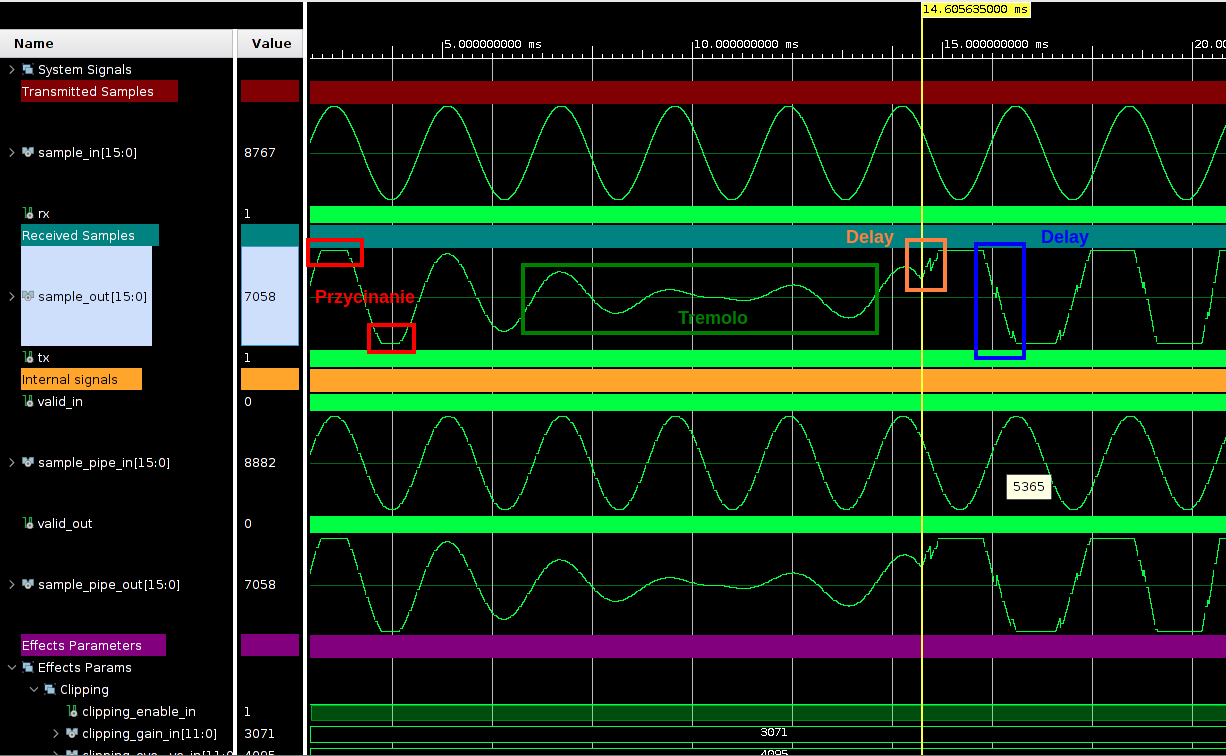
\includegraphics[width=\textwidth]{img/sim/top_all_effects_sim.png}
    \captionsetup{format=plain,justification=centering}
    \caption{Symulacja pełnego toru przetwarzania (wszystkie efekty aktywne)}
    \label{top-all-sim}
\end{figure}
\vspace{0.75cm}

Rys. \ref{top-all-sim} przedstawia symulację pełnego toru pomiarowego z~wszystkimi efektami w~stanie aktywnym. Tak jak w~przypadku poprzednich symulacji jako pobudzenie zastosowano falę sinusoidalną o~częstotliwości $440$Hz. Częstotliwość próbkowania wynosiła $44100$Hz. Sygnał \verb|sample_in| ukazuje pobudzenie wejścia urządzenia przesyłanego przez linię \verb|rx|. Z~kolei sygnał \verb|sample_out| to wyjście z~urządzenia odebrane przez jedną z~opisanych wcześniej funkcji bibliotecznych z~linii \verb|tx|. Dodatkowo zamieszczone zostały również przebiegi wewnętrznych (względem urządzenia) wartości wejściowej i~wyjściowej do potoku (t.j. wewnętrzne wyjście z~bloku odbierającego i~wejście do bloku transmitującego próbki). Na ukazanym przebiegu zaobserwować można efekty charakterystyczne dla każdgeo z~filtrów. W~pierwszej kolejności pojawia się przycinanie sygnału. Wzmocnienie modułu \textit{distortion} wynosiło $3$. W~następnej kolejności wkład do sygnału wyjściowego wnosi efekt termolo, który w~sposób cykliczny moduluje amplitudę wyjściową ze~współczynnikiem wzmocnienia w~zakresie $[0,1]$. Po $14.6$ms pojawia się skokowa zmiana sygnału wynikająca z~aktywacji modułu \textit{delay}, którego głębokość ustawiono na około $660$ próbek. Wpływ bloku \textit{flanger} nie jest tutaj widoczny, co wynika z~niewielkiego przedziału czasowego ukazanego na rysunku.
